\section{MPI quick tuning}


\chapterDescription
  {
    Around 15 minutes.
  }
  {
    A working MPI code.
  }


This section collects a couple of really primitive measurements to make your
code faster.

\subsection{Filter out log statements}

It is probably to simple to mention, but all our teams from time to time forget
this. 
One of the major things slowing down codes is writing to the terminal. 
So adding a few additional log filters can significantly speed up your code.



\subsection{Switch off load balancing}

Most of Peano's load balancing algorithms (at least the ones coming along with
the standard package) rely on a central node pool.
If a rank decides that it would be advantageous to split up its domain, it sends
a request to the first rank whether there are any idle nodes available.
If your code already uses all ranks, this is a time consuming process that
suffers from latency.
If you know a prior that the load balancing is static and no further splits of
subdomains are possible, it does make sense to switch the load balancing off.
There is a routine \texttt{activateLoadBalancing} operation on the load
balancing oracle to do so.

This operation has to be called on each individual rank, i.e.~you can switch 
the load balancing on and off on a rank-per-rank basis. There are basically two
variants/patterns to disable the load balancing:
\begin{enumerate}
  \item You may introduce a new mapping that does nothing besides switching the
  load balancing off (typically in \texttt{beginIteration}). You then merge this
  mapping into your other adapters.
  \item You add a new bool to your state. In the global runner you set this
  boolean flag once you want to switch the load balancing off. The state then is
  successively propagated to the workers. In \texttt{beginIteration}, you
  analyse this bool (in any mapping) and you switch off the load balancing if
  the flag is set.
\end{enumerate}

Peano also offers the opportunity to invoke a
global step on all ranks prior to an \texttt{iterate} call.
This feature can be used to switch off the load balancing, too:

\begin{code}
void picard::runners::Runner::runGlobalStep() {
  peano::parallel::loadbalancing::Oracle::getInstance().activateLoadBalancing(false);
}


int picard::runners::Runner::runAsMaster(...) {
  ...
  
  repository.runGlobalStep(); // on all other ranks
  runGlobalStep();            // and locally, too
}
\end{code}

\noindent
As clarified in the documentation of the operations (see the autogenerated
header files of your repository, e.g.), you have to be careful if you follow
this variant:
You are never allowed to run a global step if any rank is involved in a join or
fork. 


\subsection{Reduce data exchange with global master}

\begin{smell}
  It seems that rank 0 is involved in lots of data exchange (the performance
  analysis says that it is a neighbour data exchange bottleneck), and we see
  that rank 0 holds a significant number of total vertices and cells.
\end{smell}

Peano takes the computational Domain (the unit square, e.g.) and embeds it into
a $3^d$ patch. This surrounding patch is held by rank 0 being the global master.
This rank deploys the central element, i.e. the whole domain, immediately to
rank 1 and sticks himself with administrative duties (the node pool server
realising domain decomposition decisions, e.g.) only. 
We have a situation as sketched below on the left:

\begin{center}
  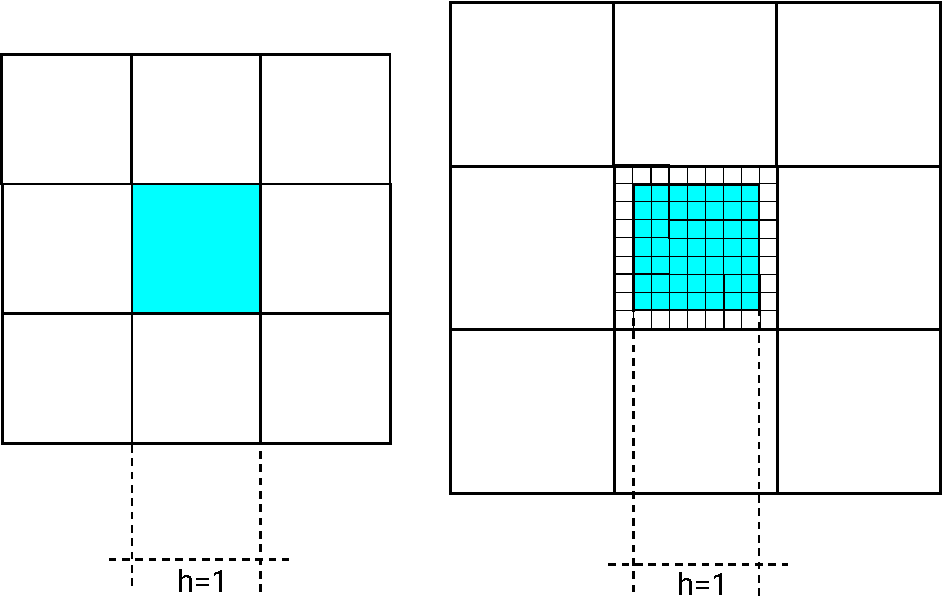
\includegraphics[width=0.5\textwidth]{62_quick-tuning/domain-layout.pdf}
\end{center}

The global master 0 deploys the real domain (filled) to rank 1 and then rank 1
continues to split up its domain further.
Though rank 0 has deployed all cells to other ranks, still many workers of rank
1 (up to eight) are adjacent to rank 0. 
If they refine (and they most probably will do as most PDE solvers refine along
the domain boundary), there is a pretty huge refined surface that connects each
of the eight workers of rank 1 with rank 0. 
And now rank 0 becomes a bottleneck though rank 0 does no computation at all.

\begin{center}
  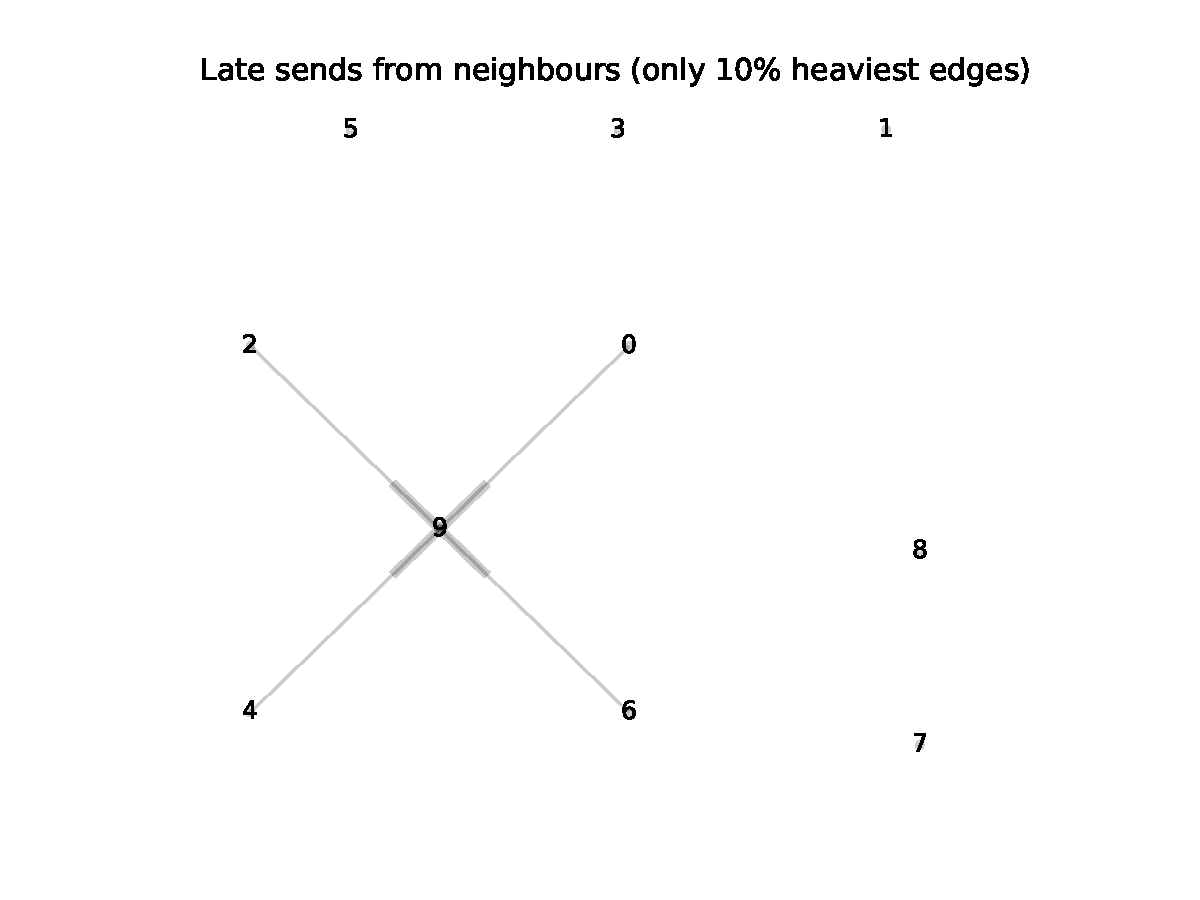
\includegraphics[width=0.45\textwidth]{62_quick-tuning/boundary-data-exchange.pdf}
  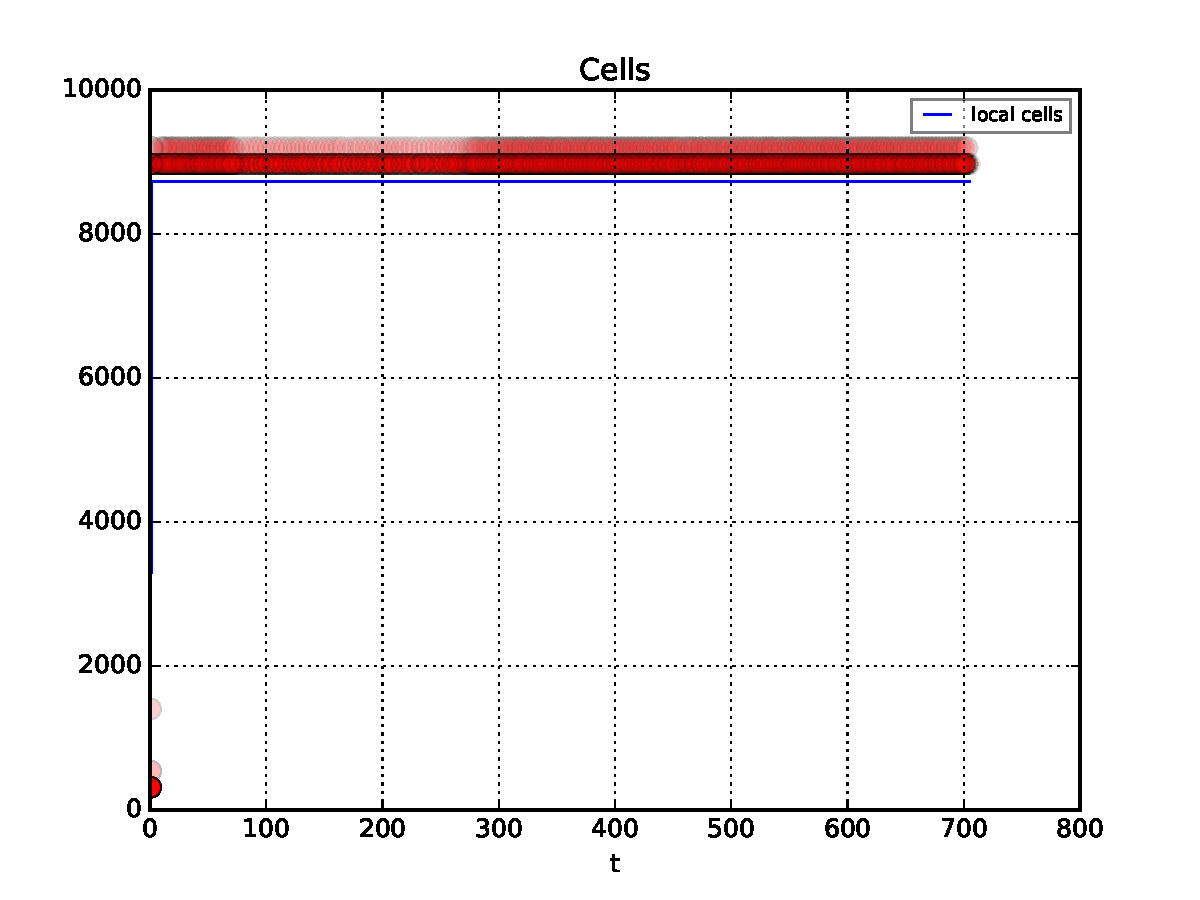
\includegraphics[width=0.45\textwidth]{62_quick-tuning/local-cells-rank-0.pdf}
  \\
\end{center}
  {
  \footnotesize
  Smells on the global master in the performance analysis output.
  Standard run on unit square, regular grid, $d=2$ with 10 ranks. 
  Left: Rank 0 is a boundary data exchange bottleneck though it has deployed all
  of its work to rank 1.
  Right:
  Rank 0 holds a significant number of cells (solid line) cmp.~to the cells on
  the other ranks (red dots) though it has deployed the domain completely.
  \vspace{0.8cm}
  
  }

One solution is to extend the bounding box around the computational domain by a
halo region.
For a unit square, using an offset of $-1/7 \times -1/7$ and a bounding box
size of $9/7 \times  9/7$ has proven of value. 
This way, all halo cells of rank 0 are sufficiently away from the domain's real
boundary. 
So, if a worker of rank 1 refines, it does not share additional Vertices with rank 0. 0 is not a bottleneck anymore.
The drawback of this approach is that the first few coarser levels on the ranks
are not involved in any computation (makes a difference for multigrid, e.g.) as
they overlap the whole computational domain. 
Only the third or fourth level of the spacetree actually holds valid compute
data.

To identify whether you can benefit from this technique, try a simple run with a
regular grid and only two ranks. 
In this case, you should not see any speedup, as all work is deployed by rank 0 to rank 1. 
However, you should also not observe a significant runtime penalty. 
If you do observe a penalty, try to realise this fix:


\begin{code}
// the actual computational domain remains the same - we are not altering the
// physics
peano::geometry::Hexahedron geometry(
  tarch::la::Vector<DIMENSIONS,double>(1.0),
  tarch::la::Vector<DIMENSIONS,double>(0.0) );
myproject::repositories::Repository* repository = 
  myproject::repositories::RepositoryFactory::getInstance().createWithSTDStackImplementation(
  geometry,
  tarch::la::Vector<DIMENSIONS,double>(9.0/7.0),   // has been 1.0 before
  tarch::la::Vector<DIMENSIONS,double>(-1.0/7.0)   // has been 0.0 before
  computationalDomainOffset );
\end{code}
